
%----------------------------------------------------------------------------------------
%	PACKAGES AND OTHER DOCUMENT CONFIGURATIONS
%----------------------------------------------------------------------------------------

\documentclass[12pt]{article} % Default font size is 12pt, it can be changed here
\usepackage{hyperref}
\usepackage{amsmath}
\usepackage{geometry} % Required to change the page size to A4
\geometry{a4paper} % Set the page size to be A4 as opposed to the default US Letter
\usepackage{longtable}
\usepackage{graphicx} % Required for including pictures
\usepackage{enumerate}
\usepackage{float} % Allows putting an [H] in \begin{figure} to specify the exact location of the figure
\usepackage{wrapfig} % Allows in-line images such as the example fish picture

\usepackage{lipsum} % Used for inserting dummy 'Lorem ipsum' text into the template

\linespread{1.2} % Line spacing

%\setlength\parindent{0pt} % Uncomment to remove all indentation from paragraphs

\graphicspath{{./Pictures/}} % Specifies the directory where pictures are stored
\begin{document}

%----------------------------------------------------------------------------------------
%	TITLE PAGE
%----------------------------------------------------------------------------------------

\begin{titlepage}

\newcommand{\HRule}{\rule{\linewidth}{0.5mm}} % Defines a new command for the horizontal lines,
%change thickness here
\center % Center everything on the page

\includegraphics[width=\textwidth]{Glasgow}\\[1.5cm]
\textsc{\LARGE Artificial Intelligence 4}\\[0.5cm] % Major heading such as course name
\textsc{\Large Assessed Exercise}\\[0.5cm] % Minor heading such as course title

\HRule \\[0.4cm]
{ \huge \bfseries Sound File Signal Processing}\\[0.4cm] % Title of your document
\HRule \\[1.5cm]

\begin{minipage}{0.4\textwidth}
\begin{flushleft} \large
\emph{Author:}\\
Garry \textsc{Sharp}\\
0801585s\\ % Your name
\end{flushleft}
\end{minipage}
~
\begin{minipage}{0.4\textwidth}
\begin{flushright} \large
\emph{Supervisors:} \\
Dr. A. \textsc{Vinciarelli}\\ % Supervisor's Name
Dr. M. \textsc{Filippone}\\ % Supervisor's Name
\end{flushright}
\end{minipage}\\[4cm]

{\large \today}\\[3cm] % Date, change the \today to a set date if you want to be precise

\vfill % Fill the rest of the page with whitespace

\end{titlepage}

%----------------------------------------------------------------------------------------
%	TABLE OF CONTENTS
%----------------------------------------------------------------------------------------

\newpage
\tableofcontents % Include a table of contents

\newpage
\section{Design}
\subsection{Performance}
The system as a whole works reasonably well, it shows 94\% accuracy overall (it makes a total of 6
incorrect guesses) and executes in 6.657 seconds real time (0.168 seconds system time). More
information regarding accuracy can be found in section \ref{sec:Accuracy} as well as other further
information related to the performance of the system (See Section \ref{sec:Experiments})
 
\subsection{Environment}
The environment for the system as it stands now is purely digital, that is to say, files that are
read from or written to. A list of manipulated files is as follows:
\begin{enumerate}[i]
  \item The silence\_x.dat files (where x is a number from 01 - 50).
  \item The speech\_x.dat file (where x is a number from 01 - 50).
  \item The charts that are created.
  \item The output print statements.
\end{enumerate}

The .dat files are of a static nature in this exercise (although in a real life system with actual
audio sensing these would be dynamic), they are also input based.

The chards and print statements are of a dynamic nature and are output based (although, for this
exercise with a static input the output is also static unless the code base is altered).

It should be noted that if raw data capture were involved in the system, that the environment could
be extended to the physical space from where the sound orininated.

\subsection{Actuators}
The system actuates upon whatever the standard output is for the console and prints to it. This
could be in the form of a .txt file, a physical sheet of paper or even the console window itself.

\subsection{Sensors}
Techninically, the sensor for the system would be the functions as part of the standard python
library that are used to read in the values of the files (as we are given the values from the files
directly). In a more expanded system, where the audio is captured and sampled within the program, a
microphone could also be considered as a sensor.
%----------------------------------------------------------------------
\newpage
\section{Theory}
\subsection{Calculating the Energy, Magnitude and ZCR}
\subsubsection{Per Window}
In the context of this specific exercise, the window size corresponds to 240 samples or 30ms (which
is 10\% of the total number of samples). 
\begin{description}
\item[Energy]\hfill \\
The energy was calculated using the following equation where w refers to the current window (of
size 240 in the system). In plain English, each of the values within the window was squared and
then summed.

\[
E[n]= \sum_{k=-\infty}^{\infty} s_k{}^2 \cdot w[n-k]
\]

\item[Magnitude]\hfill \\
The magnitude was calculated using the following equation where w refers to the current window (of
size 240 in the system). In plain English, for each value in the window, the absolute was taken and
then the values were summed.

\[
M[n]= \sum_{k=-\infty}^{\infty} |s_k| \cdot w[n-k]
\]

\item[Zero Crossing Rate (ZCR)]\hfill \\
The Zero Crossing Rate (or ZCR) was calculated using the following formula where w refers to the
rectangular window.

\[
Z[n]= \frac{1}{2N} \sum_{k=-\infty}^{\infty} |sign(s_k) - sign(s_{k-1})| \cdot w[n - m] 
\]

The function sign is as described below.

\[ sign(x) = \left\{ \begin{array}{ll}
         1 & \mbox{if $x \geq 0$};\\
         0 & \mbox{if $x < 0$}.\end{array} \right. \]

In plain English, the ZCR is calculated by taking the sign of the current value $s_k$ in the set s
and subtracting from it the sign of the value preceding it in the set ($s_{k-1}$). This value is
then absoluted. Finally all of these values are then summed and divided by two times the window
size (480 in this system).

\end{description}

\subsubsection{Per File}

The values E, M and Z for each file are calculated by taking the mean value of all of the values
for Energy, Magnitude and Zero Crossing Rate respectively. The mean is calculated in the standard
fashion as detailed in the below equation.

\[
\bar{x}= \frac{1}{n}\sum_{i=1}^{n}x_i
\] 
\subsection{K-Fold Validation}

For this system, k was equal to 10 for the k-fold validation. Below is a detailed description of
how I performed each step in the process.

\subsubsection{Permuting the Data}
The data (after having calulated the average Energy, Magnitude and Zero Crossing Rate for each
file) was stored in 3 arrays (one each for Energy, Magnitude and ZCR) of size 100. The ordering of
the array was of the pattern 
silence\_01, speech\_01, silence\_02, speech\_02 ... silence\_50, speech\_50. This meant that
removing any subset of size 10 (which would represent the test set) from the array would always
result both sets having an equal number of silence and speech files. To therefore gather the test
and training sets, I simply removed a subset of $s_i$ to $s_{i+10}$ and used it as the test set and
then used the other set as the training set. For example my first iteration's test set was from
$s_0$ to $s_9$ and the training set was $s_{10}$ to $s_{99}$. My second iteration used values
$s_{10}$ to $s_19$ as the training set and $s_0$ to $s_9$ AND $s_{20}$ to $s_{99}$ as the training
set. 


\subsection{Calculating the Mean and Variance}
This stage involves calculating 12 values as follows:
\begin{enumerate}[i]
\item The mean energy value for all silence files in the training set.
\item The mean magnitude value for all silence files in the training set.
\item The mean ZCR value for all silence files in the training set.
\item The mean energy value for all speech files in the training set.
\item The mean magnitude value for all speech files in the training set.
\item The mean ZCR value for all silence speech in the training set.

\item The variance of energy against the mean for all silence files in the training set.
\item The variance of magnitude against the mean for all silence files in the training set.
\item The variance of ZCR against the mean for all silence files in the training set.
\item The variance of energy against the mean for all speech files in the training set.
\item The variance of magnitude against the mean for all speech files in the training set.
\item The variance of ZCR against the mean for all silence speech in the training set.
\end{enumerate}

These values give us our Gaussian variables $\mathcal{N}(m,s^2)$ where the mean is m and variance is
$s^2$, which allow us to calculate probabilities (See Section \ref{Probabilities})

\subsubsection{The Mean}
The mean was calculated in the standard fashion of summing all of the values in the set and then
dividing by the total number of values in the set. This is reflected in the equation below.

\[
\bar{x}= \frac{1}{n}\sum_{i=1}^{n}x_i
\]

\subsubsection{The Variance}
The following equation was used in the calculation of the variance, where n is the number of values
(in the program itself n was always 45 as the number of values in the training set was 90 which
accounted for 45 speech files and 45 silence files). $E_i$ refers to the current value in the
training set and m is the mean. 

\[
s^2= \frac{1}{n} \sum_{i=1}^{n} (E_i - m)^2
\]
\subsection{Calculating Probabilities}
\label{Probabilities}
\subsubsection{Individually for Energy, Magnitude and ZCR}
The following equation was used to discern the probability of a file being either speech or
silence. The equation was applied for Energy, Magnitude and ZCR using both Gaussian
variables for speech and silence. 
\[
p(x) = \mathcal{N} (x|m,s^2) = \frac{1}{\sqrt{2\pi s^2}} exp \left(\frac{(x - m)^2}{2s^2} \right)
\]
\subsubsection{Per File}
Calculating an overall probability is reasonably simple, you simply multiply all of the
probabilities for silence (Energy, Magnitude and ZCR based on the silence Gaussians) and also for
speech (Energy, Magnitude and ZCR based on the speech Gaussians).

\subsubsection{Making a Guess}
The framework for guessing will take the largest overall probability (comparison between
probability of being speech and probability of being silence) as detailed above. In the very
unlikely event that the probabilities are the same, the system will guess unknown.

\newpage
\section{Experiments}
\label{sec:Experiments}

\subsection{Scatter Plots}

Below are a series of scatter plots showing the average values for Energy, Magnitude and ZCR across
all 100 files. In each scatter diagram, the solid/blue plots represent speech files whereas the
hollow/yellow plots represent silence files.

\subsubsection{Energy vs. Magnitude}
\begin{center}
  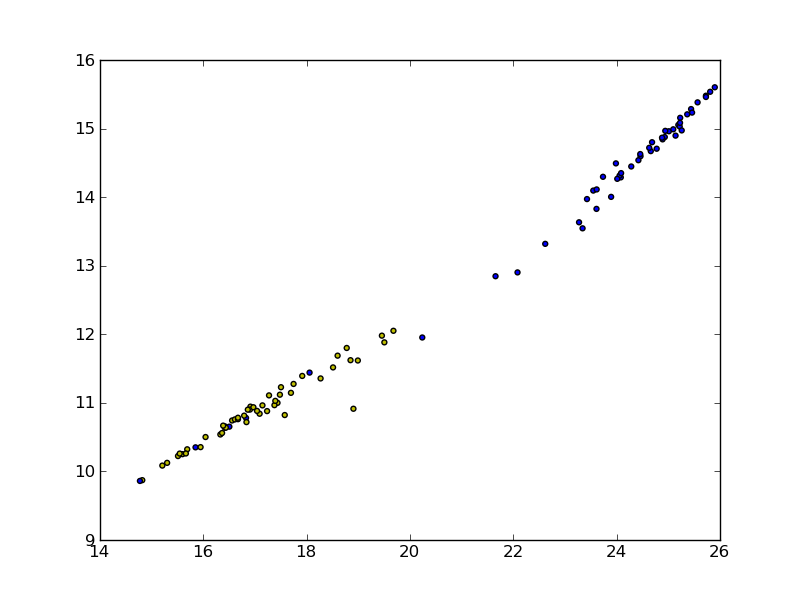
\includegraphics[width=0.75\textwidth]{eng_mag}
\end{center}
\subsubsection{Energy vs. ZCR}
\begin{center}
  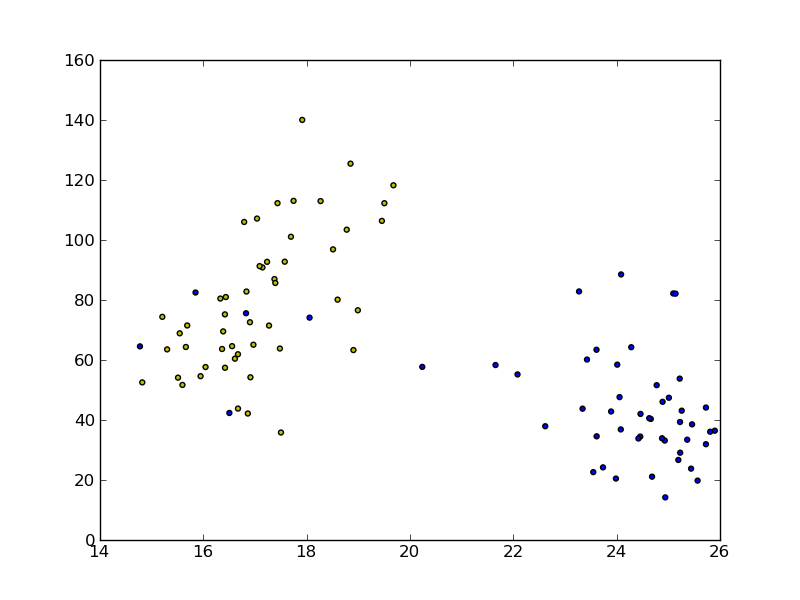
\includegraphics[width=0.75\textwidth]{eng_zcr}
\end{center}
\subsubsection{Magnitude vs. ZCR}
\begin{center}
  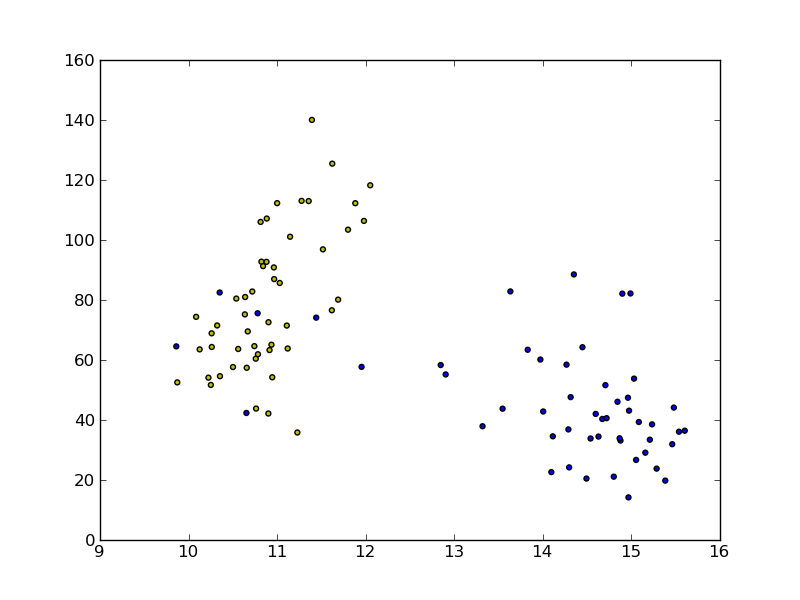
\includegraphics[width=0.75\textwidth]{mag_zcr}
\end{center}

\newpage

\subsection{Accuracy}
\label{sec:Accuracy}

\begin{table}[h]
\begin{center}
\begin{tabular}{p{0.2\textwidth} p{0.3\textwidth}}
Test Set & Percentage Accuracy \\
\hline \\
Test Set 1 & 100\% \\
Test Set 2 & 100\% \\
Test Set 3 & 90\% \\
Test Set 4 & 90\% \\
Test Set 5 & 90\% \\
Test Set 6 & 90\% \\
Test Set 7 & 100\% \\
Test Set 8 & 80\% \\
Test Set 9 & 100\% \\
Test Set 10 & 100\% \\
\end{tabular}
\caption{Showing the accuracy of the system for each test set.}
\label{TestSetStats}
\end{center}
\end{table}

\newpage
\subsection{Guesses}

The output of the system (specifically guesses) from the given input files are as follows. NB. The
actual nature of the file should alternate between silence and speech (this is known due to the
way in which files are read into the array and processed). For a list of how accurate each iteration
is please refer to Section \ref{sec:Accuracy}. In the following table, Test Set refers to the
current test iteration and File Index is the index of the test file within the scope of the Test
Set. To figure out which original file it will be

\begin{center}
\begin{longtable}{ccl}
Test Set & File Index & Guess\\
\hline \\
0&0  &SILENCE\\
0&1  &SPEECH\\
0&2  &SILENCE\\
0&3  &SPEECH\\
0&4  &SILENCE\\
0&5  &SPEECH\\
0&6  &SILENCE\\
0&7  &SPEECH\\
0&8  &SILENCE\\
0&9  &SPEECH\\
1&0  &SILENCE\\
1&1  &SPEECH\\
1&2  &SILENCE\\
1&3  &SPEECH\\
1&4  &SILENCE\\
1&5  &SPEECH\\
1&6  &SILENCE\\
1&7  &SPEECH\\
1&8  &SILENCE\\
1&9  &SPEECH\\
2&0  &SILENCE\\
2&1  &SPEECH\\
2&2  &SILENCE\\
2&3  &SPEECH\\
2&4  &SILENCE\\
2&5  &SILENCE\\
2&6  &SILENCE\\
2&7  &SPEECH\\
2&8  &SILENCE\\
2&9  &SPEECH\\
3&0  &SILENCE\\
3&1  &SILENCE\\
3&2  &SILENCE\\
3&3  &SPEECH\\
3&4  &SILENCE\\
3&5  &SPEECH\\
3&6  &SILENCE\\
3&7  &SPEECH\\
3&8  &SILENCE\\
3&9  &SPEECH\\
4&0  &SILENCE\\
4&1  &SPEECH\\
4&2  &SILENCE\\
4&3  &SPEECH\\
4&4  &SILENCE\\
4&5  &SILENCE\\
4&6  &SILENCE\\
4&7  &SPEECH\\
4&8  &SILENCE\\
4&9  &SPEECH\\
5&0  &SILENCE\\
5&1  &SPEECH\\
5&2  &SILENCE\\
5&3  &SILENCE\\
5&4  &SILENCE\\
5&5  &SPEECH\\
5&6  &SILENCE\\
5&7  &SPEECH\\
5&8  &SILENCE\\
5&9  &SPEECH\\
6&0  &SILENCE\\
6&1  &SPEECH\\
6&2  &SILENCE\\
6&3  &SPEECH\\
6&4  &SILENCE\\
6&5  &SPEECH\\
6&6  &SILENCE\\
6&7  &SPEECH\\
6&8  &SILENCE\\
6&9  &SPEECH\\
7&0  &SILENCE\\
7&1  &SPEECH\\
7&2  &SILENCE\\
7&3  &SPEECH\\
7&4  &SILENCE\\
7&5  &SPEECH\\
7&6  &SILENCE\\
7&7  &SILENCE\\
7&8  &SILENCE\\
7&9  &SILENCE\\
8&0  &SILENCE\\
8&1  &SPEECH\\
8&2  &SILENCE\\
8&3  &SPEECH\\
8&4  &SILENCE\\
8&5  &SPEECH\\
8&6  &SILENCE\\
8&7  &SPEECH\\
8&8  &SILENCE\\
8&9  &SPEECH\\
9&0  &SILENCE\\
9&1  &SPEECH\\
9&2  &SILENCE\\
9&3  &SPEECH\\
9&4  &SILENCE\\
9&5  &SPEECH\\
9&6  &SILENCE\\
9&7  &SPEECH\\
9&8  &SILENCE\\
9&9  &SPEECH\\
\end{longtable}
\end{center}

\newpage

%\begin{wrapfigure}{l}{0.5\textwidth} % Inline image example
% \begin{center}
%    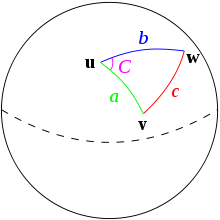
\includegraphics[width=0.42\textwidth]{haversine}
%  \end{center}
%  \parbox{0.45\textwidth}{\caption{The haversine formula calculating the true distance on the
%spherical earth}}
%\end{wrapfigure}

%----------------------------------------------------------------------------------------
%	BIBLIOGRAPHY
%----------------------------------------------------------------------------------------
\newpage
%\begin{thebibliography}{99} % Bibliography - this is intentionally simple in this template
%\bibitem
%\newblock R. W. Sinnott, "Virtues of the Haversine", Sky and Telescope 68 (2), 159 (1984).\\
%\bibitem
%\newblock HaptiMap, "Official Website", http://www.haptimap.org, accessed 25th Nov 2012 \\
%\bibitem 
%\newblock Nielsen, J., and Molich, R. (1990). Heuristic evaluation of user interfaces, Proc. ACM
%CHI'90 Conf. (Seattle, WA, 1?5 April), 249-256 \\
%\bibitem 
%\newblock John Williamson, Roderick Murray-Smith, Stephen Hughes, October 3, 2006. Excitatory
%Multimodal Interaction on Mobile Devices, accessed 25th Nov 2012 \\
%\bibitem
%\newblock Zeljko Obrenovic, Dusan Starcevic (2004), Modeling Multimodal HumanComputer Interaction,
%accessed 25th Nov 2012 \\
 
%\end{thebibliography}
\newpage
\appendix
\section{Energy, Magnitude and Zero Crossing Rate Values}
\begin{center}
\begin{longtable}{llll}
File Name & Energy & Magnitude & ZCR \\
\hline \\
 Silence 01  &  14.8181905&  9.87254156&  0.10945486\\ 
 Speech 01  &  25.7278583&  15.4791513&  0.09196527\\ 
 Silence 02  &  19.6794362&  12.0510437&  0.24633420\\ 
 Speech 02  &  24.0799154&  14.2882048&  0.07679079\\ 
 Silence 03  &  17.2338339&  10.8799228&  0.19316753\\ 
 Speech 03  &  23.2720036&  13.6332829&  0.17260590\\ 
 Silence 04  &  16.9114331&  10.9448033&  0.11299218\\ 
 Speech 04  &  25.5661937&  15.3823123&  0.04124305\\ 
 Silence 05  &  16.5566494&  10.7428855&  0.13462673\\ 
 Speech 05  &  25.0105956&  14.9606998&  0.09879687\\ 
 Silence 06  &  15.6879689&  10.3226940&  0.14898177\\ 
 Speech 06  &  25.0954392&  14.9892010&  0.17120486\\ 
 Silence 07  &  16.9020396&  10.9022325&  0.15123437\\ 
 Speech 07  &  25.8096398&  15.5366163&  0.07520225\\ 
 Silence 08  &  16.3294857&  10.5388733&  0.16766840\\ 
 Speech 08  &  23.5473281&  14.0957821&  0.04713975\\ 
 Silence 09  &  17.4355984&  11.0000529&  0.23392447\\ 
 Speech 09  &  21.6554115&  12.8465678&  0.12149652\\ 
 Silence 10  &  16.4195716&  10.6564329&  0.11961111\\ 
 Speech 10  &  25.3656362&  15.2078305&  0.06964583\\ 
 Silence 11  &  17.1440381&  10.9631978&  0.18928993\\ 
 Speech 11  &  25.2293984&  15.1569760&  0.06063194\\ 
 Silence 12  &  16.6114123&  10.7585950&  0.12591232\\ 
 Speech 12  &  23.6094617&  13.8286941&  0.13211111\\ 
 Silence 13  &  17.3765088&  10.9663581&  0.18119791\\ 
 Speech 13  &  15.8489268&  10.3512895&  0.17187065\\ 
 Silence 14  &  16.3625413&  10.5604384&  0.13265017\\ 
 Speech 14  &  23.9852958&  14.4923011&  0.04266579\\ 
 Silence 15  &  15.5957817&  10.2515114&  0.10768402\\ 
 Speech 15  &  24.7744232&  14.7061652&  0.10751822\\ 
 Silence 16  &  18.9051003&  10.9140038&  0.13189322\\ 
 Speech 16  &  16.8263386&  10.7798552&  0.15746093\\ 
 Silence 17  &  17.3932031&  11.0290752&  0.17849479\\ 
 Speech 17  &  24.4614966&  14.5967193&  0.08756076\\ 
 Silence 18  &  15.9465617&  10.3543602&  0.11376388\\ 
 Speech 18  &  23.6126359&  14.1122809&  0.07200347\\ 
 Silence 19  &  17.5757934&  10.8223510&  0.19326649\\ 
 Speech 19  &  22.0810845&  12.9025026&  0.11496961\\ 
 Silence 20  &  17.6957142&  11.1460381&  0.21060069\\ 
 Speech 20  &  24.0561433&  14.3138539&  0.09920659\\ 
 Silence 21  &  16.9692450&  10.9357291&  0.13561197\\ 
 Speech 21  &  24.9311564&  14.8764534&  0.06905729\\ 
 Silence 22  &  17.4820635&  11.1190428&  0.13298697\\ 
 Speech 22  &  24.4562097&  14.6282134&  0.07182378\\ 
 Silence 23  &  16.4179296&  10.6355416&  0.15668315\\ 
 Speech 23  &  16.5036239&  10.6530943&  0.08821267\\ 
 Silence 24  &  16.4356727&  10.6384729&  0.16873437\\ 
 Speech 24  &  24.0115100&  14.2670987&  0.12176736\\ 
 Silence 25  &  18.5988868&  11.6883026&  0.16692100\\ 
 Speech 25  &  23.7353901&  14.2967662&  0.05044010\\ 
 Silence 26  &  16.8609959&  10.9008553&  0.08784288\\ 
 Speech 26  &  23.3400119&  13.5453021&  0.09119270\\ 
 Silence 27  &  17.0892137&  10.8411649&  0.19020138\\ 
 Speech 27  &  20.2376603&  11.9532454&  0.12022569\\ 
 Silence 28  &  19.5038903&  11.8823899&  0.23388281\\ 
 Speech 28  &  25.7277238&  15.4607995&  0.06651822\\ 
 Silence 29  &  16.6708021&  10.7622438&  0.09126996\\ 
 Speech 29  &  24.2823496&  14.4471676&  0.13387586\\ 
 Silence 30  &  16.6701659&  10.7829497&  0.12899305\\ 
 Speech 30  &  24.9407110&  14.9667514&  0.02959288\\ 
 Silence 31  &  17.7464385&  11.2759219&  0.23551736\\ 
 Speech 31  &  24.8886605&  14.8427144&  0.09599565\\ 
 Silence 32  &  15.6620026&  10.2619129&  0.13403906\\ 
 Speech 32  &  25.1934854&  15.0526787&  0.05560503\\ 
 Silence 33  &  18.8485759&  11.6222199&  0.26136111\\ 
 Speech 33  &  25.4405116&  15.2844281&  0.04956597\\ 
 Silence 34  &  15.5098995&  10.2244129&  0.11274565\\ 
 Speech 34  &  24.0857221&  14.3502382&  0.18442795\\ 
 Silence 35  &  15.5430064&  10.2603319&  0.14352690\\ 
 Speech 35  &  24.8781547&  14.8666565&  0.07065017\\ 
 Silence 36  &  16.8346293&  10.7191943&  0.17256423\\ 
 Speech 36  &  25.2199826&  15.0296811&  0.11207465\\ 
 Silence 37  &  18.7751966&  11.8004094&  0.21550173\\ 
 Speech 37  &  24.6602339&  14.6711315&  0.0840625\\ 
 Silence 38  &  17.5027746&  11.2282560&  0.07465277\\ 
 Speech 38  &  23.4257651&  13.9718581&  0.12531163\\ 
 Silence 39  &  18.5105591&  11.5168204&  0.20183246\\ 
 Speech 39  &  14.7730310&  9.86140434&  0.13446354\\ 
 Silence 40  &  16.3838741&  10.6680383&  0.14486371\\ 
 Speech 40  &  18.0560317&  11.4411074&  0.15441493\\ 
 Silence 41  &  15.2990479&  10.1250974&  0.13237239\\ 
 Speech 41  &  22.6175322&  13.3189989&  0.07900347\\ 
 Silence 42  &  16.7902125&  10.8134292&  0.22086458\\ 
 Speech 42  &  25.8992214&  15.6021272&  0.07591319\\ 
 Silence 43  &  18.2692975&  11.3561345&  0.23536979\\ 
 Speech 43  &  24.4206929&  14.5383240&  0.07048784\\ 
 Silence 44  &  17.0393628&  10.8825532&  0.22322135\\ 
 Speech 44  &  25.1398304&  14.8971795&  0.17107638\\ 
 Silence 45  &  15.2062666&  10.0852154&  0.15496701\\ 
 Speech 45  &  24.6849800&  14.8009195&  0.04398090\\ 
 Silence 46  &  17.2714316&  11.1089300&  0.14891579\\ 
 Speech 46  &  23.8926520&  14.0039271&  0.08924565\\ 
 Silence 47  &  17.9142265&  11.3925960&  0.29172482\\ 
 Speech 47  &  24.6300962&  14.7194521&  0.08459201\\ 
 Silence 48  &  18.9904911&  11.6177766&  0.15953559\\ 
 Speech 48  &  25.2590496&  14.9731213&  0.0898125\\ 
 Silence 49  &  16.0427867&  10.5015867&  0.12011111\\ 
 Speech 49  &  25.4595605&  15.2331701&  0.08030729\\ 
 Silence 50  &  19.4560825&  11.9800991&  0.22160763\\ 
 Speech 50  &  25.2263110&  15.0835968&  0.08193836
\end{longtable}
\end{center}

\newpage
\section{Code}
In order to see more detail in the solution, please uncomment the sections as advised in the code.
The code requires numpy and mathplotlib to be installed in order for the graphs to be shown.
\small
\begin{verbatim}
import numpy
import math
import matplotlib.pyplot as plt
count = 1
import random


filename = ""

#Helper function
def toInt(x):
	return int(x)

#Helper function
def squares(x):
	return (x*x)

#Sign function for ZCR
def sign(x):
	if x >= 0:
		return 1
	else:
		return 0

#Helper function to calculate ZCR
def zcrFunc(theLines):
	i = 1
	theLines = [0] + map(sign, theLines)
	newvals = []
	while i < 2641:
		newvals.append(theLines[i] - theLines[i-1])
		i = i + 1
	newvals = map(abs, newvals)
	return sums(newvals)

#Helper function
def toFloat(x):
	return float(x)

#Helper sum function
def sums(ll):
	i = 0
	j = 240
	listofsums = []
	while (j < 2640):
		listofsums.append(sum(ll[i:j]))
		i = i + 1
		j = j + 1
	return listofsums

#Reads in files and calculates values of E, M and Z
def mainFunc(fileName):
	f = open(fileName,'r')
	lines = f.readlines()
	intLines = [0]*240
	intLines = intLines + map(toInt, lines)
	energy_temp = map(squares, intLines)
	magnitude_temp = map(abs, intLines)
	Z = numpy.mean(zcrFunc(intLines))/480
	E = math.log(numpy.mean(sums(energy_temp)))
	M = math.log(numpy.mean(sums(magnitude_temp)))
	listofenergy.append(E)
	listofmags.append(M)
	listofzcr.append(Z)
	print fileName + "\tE: " + str(E)[0:10] + "\tM: " + 
		      str(M)[0:10] + "\tZ: " + str(Z)[0:10]

#Breaks a list into k sub-lists
def foldbreak(k, list_x):
    endlist = []
    count = 100/k
    while (count < 110):
	upper = count
	lower = upper - (100/k)
	endlist.append(list_x[lower:upper])
	count += (100/k)
    return endlist

listofenergy = [] 
listofmags = [] 
listofzcr = []

print "\n"
while (count <= 50):
	if (count < 10):
		filename1 = "silence_speech/silence_0" + 
			  str(count) + ".dat"
		filename2 = "silence_speech/speech_0" + 
			  str(count) + ".dat"
	else:
		filename1 = "silence_speech/silence_" + 
			   str(count) + ".dat"
		filename2 = "silence_speech/speech_" + 
			    str(count) + ".dat"
	mainFunc(filename1)
	mainFunc(filename2)
	count += 1


count = 0
while (count < 100):

	plt.figure(0)
	plt.scatter(listofenergy[count],listofmags[count],s=10,c='y')
	plt.scatter(listofenergy[count+1],listofmags[count+1],s=10,c='b')


	plt.figure(1)
	plt.scatter(listofenergy[count],listofzcr[count],s=10,c='y')
	plt.scatter(listofenergy[count+1],listofzcr[count+1],s=10,c='b')

	
	plt.figure(2)
	plt.scatter(listofmags[count],listofzcr[count],s=10,c='y')
	plt.scatter(listofmags[count+1],listofzcr[count+1],s=10,c='b')


	count += 2
plt.show()

k = 10

#Breaks the array of 100 values into 2D array of 10 x 10
folded_energy = foldbreak(k,listofenergy)
folded_mags = foldbreak(k,listofmags)
folded_zcr = foldbreak(k,listofzcr)

#Function for calculating the variance
def getVariance(mean, trnset):
	count = 0
	variance_count = 0
	while (count < 45):
		variance_count += ((trnset[count] - mean) * (trnset[count] - mean))
		count += 1
	return variance_count/45

count = 0
while (count < 10):
	#The Test Sets
	test_energy = folded_energy[count]
	test_mags = folded_mags[count]
	test_zcr = folded_zcr[count]

	#The Training Sets
	training_energy = []
	training_mags = []
	training_zcr = []
	i = 0
	while (i < 10):
		if (i == count):
			i += 1
		else:
			training_energy += folded_energy[i]
			training_mags += folded_mags[i]
			training_zcr += folded_zcr[i]
			i += 1
	
	i = 0

	#Splitting the Training Set into Speech and Silence sub sets
	training_speech_energy = []
	training_silence_energy = []
	training_speech_mags = []
	training_silence_mags = []
	training_speech_zcr = []
	training_silence_zcr = []

	while (i < 90):
		training_silence_energy.append(training_energy[i])
		training_speech_energy.append(training_energy[i+1])
		training_silence_mags.append(training_mags[i])
		training_speech_mags.append(training_mags[i+1])
		training_silence_zcr.append(training_zcr[i])
		training_speech_zcr.append(training_zcr[i+1])
		i += 2
	
	#Calculating the mean value
	training_speech_mean_energy = numpy.mean(training_speech_energy)
	training_silence_mean_energy = numpy.mean(training_silence_energy)
	training_speech_mean_mags = numpy.mean(training_speech_mags)
	training_silence_mean_mags = numpy.mean(training_silence_mags)
	training_speech_mean_zcr = numpy.mean(training_speech_zcr)
	training_silence_mean_zcr = numpy.mean(training_silence_zcr)

	#Calculating the variance using custon getVariance function
	train_speech_energy_var = 
	  getVariance(training_speech_mean_energy, training_speech_energy)
	train_silence_energy_var = 
	  getVariance(training_silence_mean_energy,
training_silence_energy)
	train_speech_mags_var = 
	  getVariance(training_speech_mean_mags, training_speech_mags)
	train_silence_mags_var = 
	  getVariance(training_silence_mean_mags, training_silence_mags)
	train_speech_zcr_var = 
	  getVariance(training_speech_mean_zcr, training_speech_zcr)
	train_silence_zcr_var = 
	  getVariance(training_silence_mean_zcr, training_silence_zcr)

	
	print "------------------- Test Iteration " + str(count) + "-------------------\n\n"

	#Shows Mean and Variance Values, Uncomment if you
	#Want this to be displayed as output

	#print "training speech mean energy: " + str(training_speech_mean_energy)[:9] +
"\t\ttraining speech variance energy: " + str(train_speech_energy_var)[:9]
	#print "training silence mean energy: " + str(training_silence_mean_energy)[:9] +
"\t\ttraining silence variance energy: " + str(train_silence_energy_var)[:9] + "\n"

	#print "training speech mean mags: " + str(training_speech_mean_mags)[:9] 
	  + "\t\ttraining speech variance mags: " + str(train_speech_mags_var)[:9]
	#print "training silence mean mags: " + str(training_silence_mean_mags)[:9] 
	  + "\t\ttraining silence variance mags: " + str(train_silence_mags_var)[:9] +"\n"

	#print "training speech mean zcr: " + str(training_speech_mean_zcr)[:9] 
	  + "\t\ttraining speech variance zcr: " + str(train_speech_zcr_var)[:9]
	#print "training silence mean zcr: " + str(training_silence_mean_zcr)[:9] 
	  + "\t\ttraining silence variance zcr: " + str(train_silence_zcr_var)[:9] + "\n"
	
	i = 0;
	
	while (i < 10):

		test_val_e = test_energy[i]
		test_val_m = test_mags[i]
		test_val_z = test_zcr[i]
		pi = math.pi

		#Calculate probabilities for Energy
		prob_sil_energy = (1/math.sqrt(2 * pi *
train_silence_energy_var))*((math.exp(-(test_val_e -
training_silence_mean_energy)**2))/(2*train_silence_energy_var))
		prob_speech_energy = (1/math.sqrt(2 * pi *
train_speech_energy_var))*((math.exp(-(test_val_e -
training_speech_mean_energy)**2))/(2*train_speech_energy_var))
		
		#Calculate probabilities for Magnitude
		prob_sil_mags = (1/math.sqrt(2 * pi *
train_silence_mags_var))*((math.exp(-(test_val_m -
training_silence_mean_mags)**2))/(2*train_silence_mags_var))
		prob_speech_mags = (1/math.sqrt(2 * pi *
train_speech_mags_var))*((math.exp(-(test_val_m -
training_speech_mean_mags)**2))/(2*train_speech_mags_var))		
		
		#Calculate probabilities for ZCR

		prob_sil_zcr = (1/math.sqrt(2 * pi * train_silence_zcr_var))*
((math.exp(-(test_val_z
- training_silence_mean_zcr)**2))/(2*train_silence_zcr_var))

		prob_speech_zcr = (1/math.sqrt(2 * pi * train_speech_zcr_var))*
((math.exp(-(test_val_z -
training_speech_mean_zcr)**2))/(2*train_speech_zcr_var))
		
		#Calculate OVERALL probability
		prob_sil = prob_sil_energy * prob_sil_mags * prob_sil_zcr
		prob_speech = prob_speech_energy * prob_speech_mags * prob_speech_zcr
    
		#Prints probability values, uncomment if you
		#would like to see the values

		#print "Probability silence based on energy: " + str(prob_sil_energy)
		#print "Probability speech based on energy: " + str(prob_speech_energy)
		#print "Probability silence based on magnitude: " + str(prob_sil_mags)
		#print "Probability speech based on magnitude: " + str(prob_speech_mags)	
		#if (prob_sil_zcr == 0):
		#  print "Probability silence based on zcr too small to calculate"
		#else:
		#  print "Probability silence based on zcr: " + str(prob_sil_zcr)
		#if (prob_speech_zcr == 0):
		#  print "Probability silence based on zcr too small to calculate"
		#else:
		#  print "Probability speech based on zcr: " + str(prob_speech_zcr)

		energy_guess = ""
		mags_guess = ""
		zcr_guess = ""
		final_guess = ""

	#ENERGY
		if (prob_speech_energy > prob_sil_energy):
			energy_guess = "speech"
		elif (prob_sil_energy > prob_speech_energy):
			energy_guess = "silence"
		else:
			energy_guess = "unknown"

		#Guess based solely on ENERGY.
		#print "Guess for ENERGY \t" + str(count) + "-" + str(i) + " is \t" +
energy_guess.upper()

	#MAGNITUDE
		if (prob_speech_mags > prob_sil_mags):
			mags_guess = "speech"
		elif (prob_sil_mags > prob_speech_mags):
			mags_guess = "silence"
		else:
			mags_guess = "unknown"
		#Guess based solely on MAGNITUDE.
		#print "Guess for MAGNITUDE \t" + str(count) + "-" + str(i) + " is \t" +
mags_guess.upper()

	#ZCR
		if (prob_speech_zcr > prob_sil_zcr):
			zcr_guess = "speech"
		elif (prob_sil_zcr > prob_speech_zcr):
			zcr_guess = "silence"
		else:
			zcr_guess = "unknown"
		#Guess based solely on ZCR.
		#print "Guess for ZCR \t\t" + str(count) + "-" + str(i) + " is \t" +
zcr_guess.upper()
		
	#FINAL
		if (prob_speech > prob_sil):
			final_guess = "speech"
		elif (prob_sil > prob_speech):
			final_guess = "silence"
		else:
			final_guess = "unknown"
		print "Final Guess is \t\t" + str(count) + "-" + str(i) + " is \t" +
final_guess.upper() + "\n"
		i += 1
	count += 1

\end{verbatim}
%----------------------------------------------------------------------------------------

\end{document}